\documentclass[11pt,twocolumn]{amsart}
\setlength{\columnsep}{0.5cm}

\usepackage{amsfonts,amsthm,amssymb,amsmath,amsopn,float}
\usepackage{xifthen}
\usepackage{graphicx}
\usepackage{tikz,pgfplots}
\usepackage{epstopdf}
%\usepackage{hyperref}
\usepackage[pdftex,backref=section,hypertexnames=true,plainpages=false,
naturalnames,colorlinks=true,linkcolor=blue,bookmarks]{hyperref}
\usepackage[margin=0.5in]{geometry}  % set the margins to 1ine on all sides
%\usepackage{subfigure}
%\usepackage{subcaption}
%\usepackage[foot]{amsaddr} % to add address of the authors in footnote size at the bottom

% for more insight into compilation error
\errorcontextlines 90000
%% to check reference need to uncomment and after checking need to comment this back.
%\usepackage{refcheck} 

\usepackage{algorithm}
%\usepackage{algpseudocode}
\usepackage{algcompatible}

\usepackage{color}
\definecolor{mygray}{RGB}{47,79,79}


\usepackage{amsaddr}

\makeatletter
\renewcommand{\email}[2][]{%
	\ifx\emails\@empty\relax\else{\g@addto@macro\emails{,\space}}\fi%
	\@ifnotempty{#1}{\g@addto@macro\emails{\textrm{(#1)}\space}}%
	\g@addto@macro\emails{#2}%
}
\makeatother

\usepackage{placeins}
 	
\theoremstyle{definition}
\newtheorem{theorem}{Theorem}[section]
\newtheorem{lemma}[theorem]{Lemma}
\newtheorem{corollary}[theorem]{Corollary}
\newtheorem{proposition}[theorem]{Proposition}
\newtheorem{noname}[theorem]{}
\newtheorem{sublemma}{}[theorem]
\newtheorem{conjecture}[theorem]{Conjecture}
\newtheorem{summary}[theorem]{Summary}
\theoremstyle{definition}
\newtheorem{definition}[theorem]{Definition}
\newtheorem{example}[theorem]{Example}
\newtheorem{remark}[theorem]{Remark}
\numberwithin{equation}{section}
\newcommand{\ba}{\backslash}
\graphicspath{ {images/} }
\numberwithin{equation}{section}
\newcommand{\bolds}[1]{\boldsymbol{#1}}
\newcommand{\sref}[2]{\hyperref[#2]{#1 \ref*{#2}}}
\newcommand{\R}{\mathbf{R}}  % The real numbers.
\newcommand{\Z}{\mathbf{Z}}  % The integer numbers.


% Algorithmic modifications
%\makeatletter
%\newcommand{\HPXLOOP}[1]{\ALC@it\algorithmicloop\ #1%
%  \begin{ALC@hpx}}
%\newcommand{\ENDHPXLOOP}{\end{ALC@hpx}\ALC@it\algorithmicendloop}
%\makeatother
\algblockdefx[Hloop]{Hloop}{EndHloop}[1][]{\textbf{hpx::parallel::for$\_$loop} #1}{\textbf{end parallel for}}

\graphicspath{{imgs/}}

%-------------------------------------------------------------------------%
% document starts from here
%-------------------------------------------------------------------------%
\begin{document}
\title{Mesh partitioning for HPX parallel computing for nonlocal computational models}

\author{Prashant K. Jha$^\dagger$}


\address[$\dagger$]{Oden Institute for Computational Engineering and Sciences, \\
The University of Texas at Austin, \\
Austin, TX 78712, USA}
\email[$\dagger$]{pjha.sci@gmail.com}

\author{Patrick Diehl$^\ddagger$}

\address[$\ddagger$]{Center for Computation and Technology, \\
	Louisiana State University, \\
	Baton Rouge, LA 70803 USA}
\email[$\ddagger$]{pdiehl@cct.lsu.edu}

\maketitle

In this document, we consider a general class of nonlocal computational model seen in various fields, such as Peridynamics \cite{CMPer-Silling5,BobaruHu,HaBobaru,CMPer-Agwai,CMPer-Ghajari,Diehl,CMPer-Lipton2,CMPer-JhaLipton2,CMPer-JhaLipton5}, discrete element method \cite{NM-Desai,NM-Desai2,NM-Gladkyy,NM-Lobo,NM-Dosta}, Peridynamics plus discrete element method for granular media \cite{NM-Zhu, NM-Masoud}, nonlocal cell-cell adhesion in computational biology \cite{armstrong2006continuum,engwer2017structured,stinner2014global}, nonlocal heat equation \cite{burch2011classical,du2012analysis}. References above are only minuscule fraction of what is available. The application of nonlocal modeling method for understanding of complex spatially multiscale phenomenon is seen in various new fields such as fluid mechanics, particulate media, directed self-assembly of Block-Copolymers, tumor modeling, etc. What is more interesting and also convenient is that underlying algorithm which is used to numerically solve these nonlocal models is more or less same and therefore the efficient computational method available for one type of nonlocal model can be easily applied to the nonlocal model in other fields.

It is our understanding that efficient computational method to solve the nonlocal model is very important. It is widely known that the nonlocal models are much more computationally demanding compared to their counterpart, namely local models (such as heat equation, wave equation, etc). This is because the length of interaction in nonlocal model is typically 3 to 10 times larger than the size of discretization and therefore, the usual local assembly of matrix and vector considered in solution of pdes (partial differential equation) is not feasible. The efficient parallel implementation because of long-range interaction is difficult due to dependence over much larger length scale. 

In this document we present this problem using simple example of nonlocal diffusion equation, see \cite{burch2011classical} and references therein for more information. Our main goal is to highlight key difficulties in designing massively parallel scheme for nonlocal models while keeping the model related complexity to minimum. For this purpose nonlocal heat equation is suitable. Further, to fix the ideas we only consider two dimensional setting. 

In this work we use parallel API called HPX. HPX is an open source asynchronous many task run time system that focuses on high performance computing~\cite{Heller2017,tabbal2011preliminary,kaiser2014hpx}. HPX provides wait-free asynchronous execution and futurization for synchronization. It also features parallel execution policies utilizing a task scheduler, which enables a fine-grained load balancing parallelization and synchronization due to work stealing. HPX is in strict adherence to the C++ $11$~\cite{cxx11_standard} and C++ $17$ standard definitions~\cite{cxx17_standard}.\\


\section{Nonlocal diffusion equation}
In this section we give brief overview of nonlocal diffusion equation for temperature field $u$ over an square domain $D = [0,1]^2$ subjected to zero temperature condition on its boundary and subjected to given heat source distribution within the domain. It is a first order transient equation in time. For simplification, we only consider explicit time integration scheme, namely forward Euler scheme. For spatial discretization, we consider uniform mesh over domain $D$ and consider finite difference approximation (also commonly referred to as particle discretization). The resulting final equations are very simple and serial implementation requires only few lines of code, see \autoref{alg:serial}. With HPX, thread-level parallel implementation and shared-memory parallel implementation is almost as simple as serial implementation, see \autoref{alg:semi parallel}. 

Our goal is to fully parallelize the solver, i.e. starting from mesh partition to computation of fields at mesh nodes. We proceed step wise starting from serial implementation, to shared-memory parallel implementation, and to fully parallel implementation and discuss the challenges going from one step to next. 

Let material domain is $D = [0,1]^2$ and time domain $I = [0,T]$. We fix size of horizon (length over one point interacts with another, also called nonlocal length scale) $\epsilon>0$. Let $D_c = (-\epsilon, 1+\epsilon)^2 - D$ be the nonlocal boundary of thickness $\epsilon$ surrounding $D$. See \autoref{fig:domain}. We define $H_r(x)$ as two-dimensional open ball of radius $r$ centered at $x\in \R^2$.

\begin{figure}
\centering
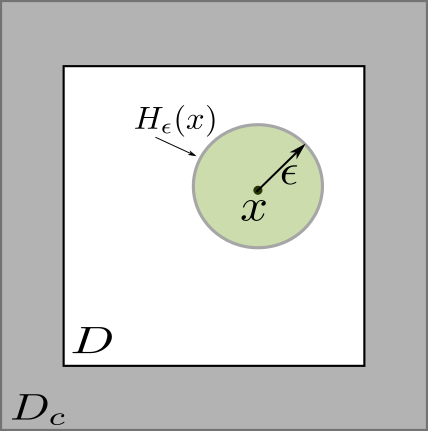
\includegraphics[scale=0.5]{material_domain.png}
\caption{Material domain $D$ and nonlocal boundary $D_c$. Figure shows typical material point $x\in D$ and ball $H_\epsilon(x)$. }\label{fig:domain}
\end{figure}

Let $u:I \times D\cup D_c \to \R$ is a temperature field. Let $J:\R \to \R$ be positive function such that $0\leq J(r) \leq M$ for $r\in [0,1]$ and $J(r) = 0$ for $r\notin [0,1]$. We refer to $J$ as influence function. 

$u(t,x)$ satisfies following nonlocal diffusion equation, $\forall x\in D \text{ and } \forall t \in I$,
\begin{align}\label{eq:diff eqn}
\dfrac{\partial }{\partial t} u(t,x) &= c \int_{H_\epsilon(x)} J(|y-x|/\epsilon) (u(t,y) - u(t,x)) dy .
\end{align}
Initial condition is given by
\begin{align}\label{eq:ic}
u(0,x) = u_0(x) \qquad \forall x\in D
\end{align}
and boundary condition is given by
\begin{align} \label{eq:bc}
u(t,x) = 0 \qquad \forall x\in D_c \text{ and } \forall t\in I.
\end{align}

Constant $c$ is chosen such that in the limit $\epsilon\to 0$ the nonlocal operator in right-hand side of \autoref{eq:diff eqn}. goes to $k\nabla \cdot \nabla u$. Local diffusion equation is given by
\begin{align}\label{eq:locdiff}
\dfrac{\partial }{\partial t} u(t,x) &= k \nabla \cdot \nabla u(t,x),
\end{align}
where $k$ is the diffusivity constant. Boundary condition is $u = 0$ on $\partial D$ (consistent with boundary condition in \autoref{eq:bc} and initial condition is $u(0,x) = u_0(x)$. Constant $c$ is taken as
\begin{align}\label{eq:constc}
c &:= \begin{cases}
\frac{k}{\epsilon^3 M_2}, \qquad \text{when dimension }d=1 \\
\frac{k}{\pi\epsilon^4 M_3}, \qquad \text{when dimension }d=2,
\end{cases}
\end{align}
where 
\begin{align}\label{eq:momentJ}
M_i = \int_0^1 J(r) r^i dr.
\end{align}
For standard influence functions, $M_i$ can be computed easily. For example, when $J = 1$, $M_i = 1/(i+1)$, when $J = 1- r$, $M_2 = 1/12, M_3 = 1/20$, etc.

With choice of constant $c$ in \autoref{eq:constc}, it can be shown formally that
\begin{align}\label{eq:limit}
c \int_{H_\epsilon(x)} J(|y-x|/\epsilon) (u(t,y) - u(t,x)) dy \to k \nabla \cdot \nabla u(t,x).
\end{align}

% Insert the algorithm
\begin{algorithm}[ht]
	\caption{Serial implementation}
	\label{alg:serial}
	\begin{algorithmic}[1]
		\STATE \textcolor{mygray}{\it $\%$ Create neighbor list}
		\FOR {each integer $i \in K$}
			\IF {$|x_i - x_j| \leq \epsilon$}
				\STATE Add $j$ to neighborList$[i]$
			\ENDIF
		\ENDFOR
		\STATE
		\STATE \textcolor{mygray}{\it $\%$ $U$ is the vector of temperatures of}
		\STATE \textcolor{mygray}{\it $\%$ all mesh nodes.}
		\STATE
		\STATE \textcolor{mygray}{\it $\%$ integrate in time}
		\FOR {each integer $0\leq k \leq T/\Delta t$}
			\STATE \textcolor{mygray}{\it $\%$ time step $k$}
			\FOR {each integer $i \in K$}
				\STATE \textcolor{mygray}{\it $\%$ Loop over neighbors of $i$}
				\STATE $val\_i = 0$
				\FOR {each integer $j\in$ neighborList$[i]$}
					\STATE $val\_i = val\_i + $					
					\STATE $\quad c J(|x_j - x_i|/\epsilon) (U[j] - U[i])V_j$
				\ENDFOR
				\STATE \textcolor{mygray}{\it $\%$ Update temperature}
				\STATE $U[i] = U[i] + \Delta t \times val\_i$
			\ENDFOR	
			\STATE \textcolor{mygray}{\it $\%$ Output temperature at time $t^k = k\Delta t$}
			\STATE Output($U$)
		\ENDFOR
	\end{algorithmic}
\end{algorithm}

\section{Finite difference approximation}
Consider uniform mesh $D_h = (D\cup D_c)\cap (h\Z)^2$ of mesh size $h >0$, see \autoref{fig:mesh fd}. $\Z$ is the set of positive and negative integers. Let $\Delta t$ is size of time step and $[0,T]\cap (\Delta t \Z)$ be the discretization of time domain. We assume $\epsilon = m h$ where $m\geq 1$ is some integer.

We consider index set $K \subset \Z^2$ such that for $i\in K$, $x_i = h i \in D$. Similarly, consider index set $K_c \subset \Z^2$ such that for $i\in K_c$, $x_i = h i \in D_c$.

Let $\hat{u}^k_i$ be the solution of forward Euler discretization in time. It satisfies,$\forall 1\leq k \leq T/\Delta t, \forall i \in K$,
\begin{align}\label{eq:forward fd}
\dfrac{\hat{u}^{k+1}_i - \hat{u}^k_i}{\Delta t} = c \sum_{\substack{j \in K\cup K_c,\\
|x_j-x_i| \leq \epsilon}} J(|x_j - x_i|/\epsilon) (\hat{u}^k_j - \hat{u}^k_i) V_j
\end{align}
and
\begin{align}
\hat{u}^k_i = 0 \qquad \forall 0\leq k \leq T/\Delta t, \forall i \in K_c.
\end{align}
At $k=0$, we have $\hat{u}^0_i = u_0(x_i)$ for all $i\in K$. $V_j$ is the volume occupied by node $j$ and in our case we have $V_j = h^2$. 

\begin{figure}[ht]
\centering
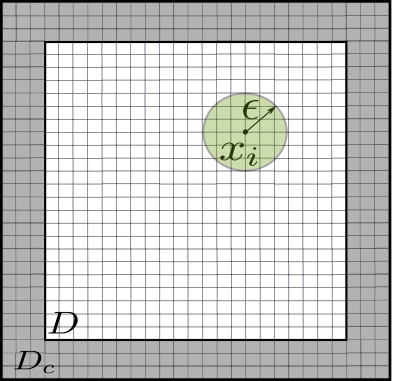
\includegraphics[scale=0.6]{mesh_uniform.png}
\caption{Uniform mesh of size $h$. Shaded area corresponds to nonlocal boundary $D_c$. We specify zero temperature on all the mesh nodes in the shaded area. For mesh node $x_i$ in $D$, we consider interaction of $x_i$ with all the mesh nodes inside the green shaded ball.}\label{fig:mesh fd}
\end{figure}



\subsection{Serial and semi-parallel implementation of forward euler scheme}
Algorithm for  serial implementation is given in \sref{Algorithm}{alg:serial}. For parallel implementation, we will use parallel for loop (HPX utility). See \sref{Algorithm}{alg:semi parallel}. In \sref{Algorithm}{alg:semi parallel}, we observe that temperature data of all mesh nodes is stored in single data variable, ``$U$", and similarly, neighbor list of all the mesh nodes are stored in single data variable, ``neighborList". We refer to this as semi-parallel as we have only parallelized for-loop and not the data. In fully parallel implementation, data will also be divided in number of computational nodes and each computational node will own data corresponding to it. This requires mesh partition. We discuss this in next section. 

% Insert the algorithm
\begin{algorithm}[ht]
	\caption{Semi-parallel implementation}
	\label{alg:semi parallel}
	\begin{algorithmic}[1]
		\STATE \textcolor{mygray}{\it $\%$ Create neighbor list using }
		\STATE \textcolor{mygray}{\it $\%$ hpx parallel for loop}
		\Hloop {each integer $i \in K$} \textbf{do}
			 \IF {$|x_i - x_j| \leq \epsilon$}
				\STATE Add $j$ to neighborList$[i]$
			\ENDIF
		\EndHloop
		\STATE
		\STATE \textcolor{mygray}{\it $\%$ is the vector of temperatures of}
		\STATE \textcolor{mygray}{\it $\%$ all mesh nodes. }
		\STATE
		\STATE \textcolor{mygray}{\it $\%$ integrate in time}
		\FOR {each integer $1\leq k \leq T/\Delta t$}
			\STATE \textcolor{mygray}{\it $\%$ time step $k$}
			\STATE \textcolor{mygray}{\it $\%$ process mesh nodes in parallel}
			\Hloop {each integer $i \in K$}
				\STATE  \textcolor{mygray}{\it $\%$ Loop over neighbors of $i$}
				\STATE $val\_i = 0$
				\FOR {each integer $j\in$ neighborList$[i]$}
					\STATE $val\_i = val\_i + $
					\STATE $\quad +  c J(|x_j - x_i|/\epsilon) (U[j] - U[i])V_j$
				\ENDFOR
				\STATE \textcolor{mygray}{\it $\%$ Update temperature}
				\STATE $U[i] = U[i] + \Delta t \times val\_i$
			\EndHloop	
			\STATE \textcolor{mygray}{\it $\%$ Output temperature at time $t^k = k\Delta t$}
			\STATE Output($U$)
		\ENDFOR
	\end{algorithmic}
\end{algorithm}

\section{Parallelization and mesh partition}
Given $N$ number of computational nodes, mesh will be partitioned in $N$ parts such that each computational node will store the information corresponding to the mesh partition it owns. For example, consider 4 computers connected by network. We would like to run the problem on all 4 computers in parallel. We will partition the mesh in four parts, see \autoref{fig:mesh partition}.

\begin{figure}
\centering
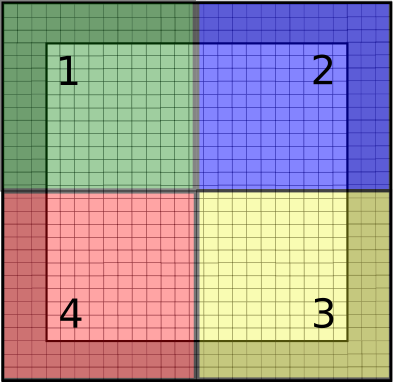
\includegraphics[scale=0.6]{mesh_partition.png}
\caption{Typical mesh partition. Mesh nodes under each color are owned by the respective computer.}\label{fig:mesh partition}
\end{figure}

In \autoref{fig:mesh partition}, the mesh is colored to show the partition. Consider part of mesh colored as green. Let us suppose the id of computer who owns the green, blue, yellow, and red are 1, 2, 3, and 4 respectively. We now focus on one computational node, say green, and present two possible situations.

\textbf{Case 1: }Consider mesh node $x_i$ which belongs to computer 1's partition. Let us suppose that $x_i$ is within the dashed line, see \autoref{fig:green case 1}. For such $x_i$, all mesh nodes $x_j \in H_\epsilon(x_i)$  will be within the green partition. Since computer 1 owns the mesh data of green partition, calculation of right hand side of \autoref{eq:forward fd}, i.e. $c J(|x_j - x_i|/\epsilon)(\hat{u}^k_j - \hat{u}^k_i)V_j$, can be carried out without needing to interact with other computers. 

\begin{figure}[ht]
\centering
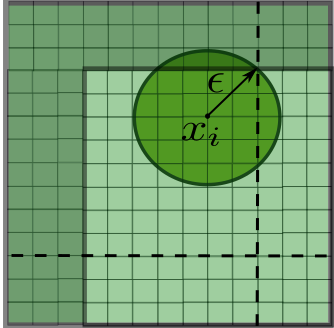
\includegraphics[scale=0.5]{mesh_partition_green_case_1.png}
\caption{Mesh nodes of green partition which are within dashed line do not interact with partition owned by other computers.}\label{fig:green case 1}
\end{figure}

\textbf{Case 2: }Now consider another mesh node $x_i$ in green partition. This mesh node is close to the boundary of green partition, and we see that there are mesh nodes $x_j$ which are in ball $H_\epsilon(x_i)$, but which are not part of green partition. For example, we consider $x_j \in H_\epsilon(x_i)$ in \autoref{fig:green case 2}. Mesh node $x_j$ is in Blue partition. Blue partition is owned by computer 2. Therefore, to compute the right hand side term in \autoref{eq:forward fd}, computer 1 has to request the information associated to mesh node $x_j$ from computer 2. We see that for all the mesh nodes in Green partition which are outside dash line, computer 1 will have to communicate with other computers for the information. 

\begin{figure}[ht]
\centering
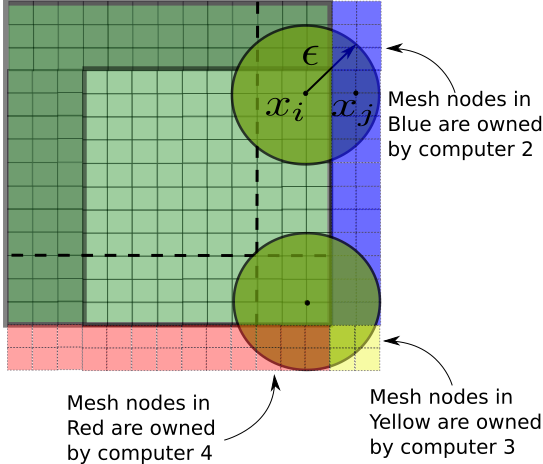
\includegraphics[scale=0.5]{mesh_partition_green_case_2.png}
\caption{In first example, mesh node $x_i$ of Green partition interacts with few mesh nodes of Blue partition owned by computer 2. In second example, we see that $x_i$ of Green mesh interacts with mesh nodes owned by computer 2, 3, and 4.}\label{fig:green case 2}
\end{figure}

\subsection{Algorithm for fully parallel code}
Consider \sref{Algorithm}{alg:parallel} which outlines the steps needed to run the problem in fully parallel framework. Following are the list of steps which will require effort in implementing \sref{Algorithm}{alg:parallel}.

\noindent \textbf{1. Partitioning of mesh: }Libraries are available which can partition the mesh into given number of computational nodes.

\noindent \textbf{2. List of interacting mesh nodes owned by other computational node: }If global mesh data is available to each computational node then we can create a list of interacting neighboring mesh nodes which are owned by other computational node. This list will have global id, which is unique, of mesh nodes. 

\noindent \textbf{3. Sharing of information: }For given computational node, we need to implement the method which shares information to other computational node and which receives the information from other computational node. For this we need a list of information to be shared and communication method available in HPX framework.


% Insert the algorithm
\begin{algorithm}[ht]
	\caption{Fully parallel implementation}
	\label{alg:parallel}
	\begin{algorithmic}[1]
		\STATE \textcolor{mygray}{\it $\%$ mesh$\_$file is the file containing mesh data}
		\STATE \textcolor{mygray}{\it $\%$ N is the number of computational nodes}
		\STATE
		\STATE \textcolor{mygray}{\it $\%$ get the id of this computational node }
		\STATE my$\_$id = get$\_$id()
		\STATE
		\STATE \textcolor{mygray}{\it $\%$ read mesh data and create mesh partition}
		\STATE myMeshNodes = create$\_$mesh$\_$partition(mesh$\_$file)
		\STATE
		\STATE \textcolor{mygray}{\it $\%$ create neighbor list.}
		\STATE neighborList = create$\_$neighbor$\_$list(mesh$\_$file)
		\STATE
		\STATE \textcolor{mygray}{\it $\%$ next task is to create a list of mesh}
		\STATE \textcolor{mygray}{\it $\%$ nodes, associated to other computational} 
		\STATE \textcolor{mygray}{\it $\%$ nodes, which interact with mesh nodes}
		\STATE \textcolor{mygray}{\it $\%$ owned by this computational node}
		\FOR {each integer $0\leq i \leq N$} 
			\IF {$i == $ my$\_id$}
				\STATE \textcolor{mygray}{\it $\%$ skip this i}
			\ELSE
				\STATE \textcolor{mygray}{\it $\%$ create a list of interacting nodes}
				\STATE \textcolor{mygray}{\it $\%$ owned by comp. node $i$}
				\STATE neighborsOutside[i] 
				\STATE \; = create$\_$list$\_$interacting$\_$nodes(my$\_$id, i)			
			\ENDIF
		\ENDFOR
		\STATE
		\STATE \textcolor{mygray}{\it $\%$ $U$ is the vector of temperatures of}
		\STATE \textcolor{mygray}{\it $\%$ mesh nodes owned by this comp. node}
		\STATE 
		\STATE \textcolor{mygray}{\it $\%$ integrate in time}
		\FOR {each integer $0\leq k \leq T/\Delta t$}
			\STATE \textcolor{mygray}{\it $\%$ time step $k$}
			\STATE 
			\STATE \textcolor{mygray}{\it $\%$ get data from other computer }
			\STATE \textcolor{mygray}{\it $\%$ before integrating in time}
			\FOR {each integer $0\leq i \leq N$} 
				\IF {$i == $ my$\_id$}
					\STATE \textcolor{mygray}{\it $\%$ skip this i}
				\ELSE
					\STATE \textcolor{mygray}{\it $\%$ request data from comp. node i}
					\STATE getData[i] = request$\_$data(my$\_$id, i)
					\STATE 
					\STATE \textcolor{mygray}{\it $\%$ share data to comp. node i}
					\STATE \textcolor{mygray}{\it $\%$ as comp. node i may also have}
					\STATE \textcolor{mygray}{\it $\%$ mesh nodes which have neighbors }
					\STATE \textcolor{mygray}{\it $\%$ in this comp. node}
					\STATE share$\_$data(my$\_$id, i)
				\ENDIF
			\ENDFOR
			\algstore{myalg}
	\end{algorithmic}
\end{algorithm}			

\begin{algorithm}
	\begin{algorithmic}[1]
	\algrestore{myalg}	
			\STATE \textcolor{mygray}{\it $\%$ we now have all the relevant data so}
			\STATE \textcolor{mygray}{\it $\%$ we can solve for temperature}
			\STATE \textcolor{mygray}{\it $\%$ at next time step}
			\Hloop {$i \in $ myMeshNodes} \textbf{do}
				\STATE \textcolor{mygray}{\it $\%$ Loop over neighbors of $i$}
				\STATE $val\_i = 0$
				\FOR {each integer $j\in$ neighborList$[i]$}
					\STATE \textcolor{mygray}{\it $\%$ check if $j$ is in myMeshNode}
					\IF {$j \in $ myMeshNode}
						\STATE \textcolor{mygray}{\it $\%$ this mesh node is within dashed line}
						\STATE
						\STATE \textcolor{mygray}{\it $\%$ compute contribution}
						\STATE $val\_i = val\_i $
						\STATE $\quad +  c J(|x_j - x_i|/\epsilon)$
						\STATE $\quad (U[j] - U[i])V_j$
					\ELSE 
						\STATE \textcolor{mygray}{\it $\%$ this mesh node is outside dashed line}
						\STATE \textcolor{mygray}{\it $\%$ search and find which comp. node }
						\STATE \textcolor{mygray}{\it $\%$ owns mesh node $j$}
						\STATE get$\_$comp$\_$id = 
						\STATE \; search$\_$for$\_$mesh$\_$node(my$\_$id, j)
						\STATE
						\STATE \textcolor{mygray}{\it $\%$ Look for j in getData[get$\_$comp$\_$id]}
						\STATE \textcolor{mygray}{\it $\%$ and get the temperature of mesh node j}			
						\STATE t$\_$j = find$\_$in(j, getData[get$\_$comp$\_$id])
						\STATE
						\STATE \textcolor{mygray}{\it $\%$ compute contribution}
						\STATE $val\_i = val\_i $
						\STATE $\quad +  c J(|x_j - x_i|/\epsilon)$
						\STATE $\quad (t\_j - U[i])V_j$	
					\ENDIF
				\ENDFOR
				\STATE \textcolor{mygray}{\it $\%$ Update temperature}
				\STATE $U[i] = U[i] + \Delta t \times val\_i$
			\EndHloop	
			\STATE \textcolor{mygray}{\it $\%$ Output temperature at time $t^k = k\Delta t$}
			\STATE Output($U$)
		\ENDFOR
	\end{algorithmic}
\end{algorithm}

\section{Constructing exact solution}
In this section we show how to construct exact solution to test the numerical results. Recall that nonlocal diffusion equation is given by 
\begin{align*}
\dfrac{\partial }{\partial t} u(t,x) &= c \int_{H_\epsilon(x)} J(|y-x|/\epsilon) (u(t,y) - u(t,x)) dy ,
\end{align*}
where $u$ is the temperature field, $c$ is a constant given by \autoref{eq:constc}. $u$ satisfies boundary condition \autoref{eq:bc} and initial condition \autoref{eq:ic}. We modify above equation to include the external source $b$:
\begin{align}\label{eq:diff eqn 2}
\dfrac{\partial }{\partial t} u(t,x) &= c \int_{H_\epsilon(x)} J(|y-x|/\epsilon) (u(t,y) - u(t,x)) dy + b(t,x).
\end{align}

\subsection{One dimension}
Let $$w(t,x) = \cos(2\pi t) \sin(2\pi x)$$ when $x\in [0,1]$ and $w(t,x) = 0$ when $x\notin [0,1]$. We want solution of \autoref{eq:diff eqn 2} $u$ to be equal to $w$, i.e., $u = w$. To achieve this we substitute 
\begin{align}\label{eq:source exact}
b(t,x) = \dfrac{\partial }{\partial t} w(t,x) -  c \int_{H_\epsilon(x)} J(|y-x|/\epsilon) (w(t,y) - w(t,x)) dy 
\end{align}
in \autoref{eq:diff eqn 2} and prescribe $u(0,x) = w(0,x) = \sin(2\pi x)$ as initial condition on $u$ and $u(t,x) = 0$ on $x\in D_c$ as boundary condition. 

\subsection{Two dimension}
Let $$w(t,x) = \cos(2\pi t) \sin(2\pi x_1)  \sin(2\pi x_2)$$ when $x\in [0,1]^2$ and $w(t,x) = 0$ when $x\notin [0,1]^2$. We want solution of \autoref{eq:diff eqn 2} $u$ to be equal to $w$, i.e., $u = w$. To achieve this we substitute 
\begin{align}\label{eq:source exact}
b(t,x) = \dfrac{\partial }{\partial t} w(t,x) -  c \int_{H_\epsilon(x)} J(|y-x|/\epsilon) (w(t,y) - w(t,x)) dy 
\end{align}
in \autoref{eq:diff eqn 2} and prescribe $$u(0,x) = w(0,x) = \sin(2\pi x_1)\sin(2\pi x_2)$$ as initial condition on $u$ and $u(t,x) = 0$ on $x\in D_c$ as boundary condition. 

%%%%%%%%%%%%%%%%%%%%%%%%%%%%%%%%%%%%%%%%%%%%%%%%%%%%%%%%%%%%%
%% References
%%%%%%%%%%%%%%%%%%%%%%%%%%%%%%%%%%%%%%%%%%%%%%%%%%%%%%%%%%%%%
\FloatBarrier
%\bibliographystyle{plain}
%\bibliography{main}

\newcommand{\noopsort}[1]{}
\begin{thebibliography}{10}
	
	\bibitem{CMPer-Agwai}
	Abigail Agwai, Ibrahim Guven, and Erdogan Madenci.
	\newblock Predicting crack propagation with peridynamics: a comparative study.
	\newblock {\em International journal of fracture}, 171(1):65--78, 2011.
	
	\bibitem{armstrong2006continuum}
	Nicola~J Armstrong, Kevin~J Painter, and Jonathan~A Sherratt.
	\newblock A continuum approach to modelling cell--cell adhesion.
	\newblock {\em Journal of theoretical biology}, 243(1):98--113, 2006.
	
	\bibitem{NM-Masoud}
	Masoud Behzadinasab, Tracy~J Vogler, Amanda~M Peterson, Rezwanur Rahman, and
	John~T Foster.
	\newblock Peridynamics modeling of a shock wave perturbation decay experiment
	in granular materials with intra-granular fracture.
	\newblock {\em Journal of Dynamic Behavior of Materials}, 4(4):529--542, 2018.
	
	\bibitem{BobaruHu}
	Florin Bobaru and Wenke Hu.
	\newblock The meaning, selection, and use of the peridynamic horizon and its
	relation to crack branching in brittle materials.
	\newblock {\em International journal of fracture}, 176(2):215--222, 2012.
	
	\bibitem{burch2011classical}
	Nathanial Burch and Richard Lehoucq.
	\newblock Classical, nonlocal, and fractional diffusion equations on bounded
	domains.
	\newblock {\em International Journal for Multiscale Computational Engineering},
	9(6), 2011.
	
	\bibitem{NM-Desai}
	Prathamesh Desai.
	\newblock Tribosurface interactions involving particulate media with
	dem-calibrated properties: Experiments and modeling.
	\newblock 2017.
	
	\bibitem{NM-Desai2}
	Prathamesh~S Desai, Akash Mehta, Patrick~SM Dougherty, and Fred~C Higgs.
	\newblock A rheometry based calibration of a first-order dem model to generate
	virtual avatars of metal additive manufacturing (am) powders.
	\newblock {\em Powder technology}, 342:441--456, 2019.
	
	\bibitem{Diehl}
	P~Diehl, R~Lipton, and MA~Schweitzer.
	\newblock Numerical verification of a bond-based softening peridynamic model
	for small displacements: Deducing material parameters from classical linear
	theory.
	\newblock 2016.
	
	\bibitem{NM-Dosta}
	Maksym Dosta, Steven Dale, Sergiy Antonyuk, Carl Wassgren, Stefan Heinrich, and
	James~D Litster.
	\newblock Numerical and experimental analysis of influence of granule
	microstructure on its compression breakage.
	\newblock {\em Powder technology}, 299:87--97, 2016.
	
	\bibitem{du2012analysis}
	Qiang Du, Max Gunzburger, Richard~B Lehoucq, and Kun Zhou.
	\newblock Analysis and approximation of nonlocal diffusion problems with volume
	constraints.
	\newblock {\em SIAM review}, 54(4):667--696, 2012.
	
	\bibitem{engwer2017structured}
	Christian Engwer, Christian Stinner, and Christina Surulescu.
	\newblock On a structured multiscale model for acid-mediated tumor invasion:
	the effects of adhesion and proliferation.
	\newblock {\em Mathematical Models and Methods in Applied Sciences},
	27(07):1355--1390, 2017.
	
	\bibitem{CMPer-Ghajari}
	M~Ghajari, L~Iannucci, and P~Curtis.
	\newblock A peridynamic material model for the analysis of dynamic crack
	propagation in orthotropic media.
	\newblock {\em Computer Methods in Applied Mechanics and Engineering},
	276:431--452, 2014.
	
	\bibitem{NM-Gladkyy}
	Anton Gladkyy and Meinhard Kuna.
	\newblock Dem simulation of polyhedral particle cracking using a combined
	mohr--coulomb--weibull failure criterion.
	\newblock {\em Granular Matter}, 19(3):41, 2017.
	
	\bibitem{HaBobaru}
	Youn~Doh Ha and Florin Bobaru.
	\newblock Studies of dynamic crack propagation and crack branching with
	peridynamics.
	\newblock {\em International Journal of Fracture}, 162(1-2):229--244, 2010.
	
	\bibitem{Heller2017}
	Thomas Heller, Patrick Diehl, Zachary Byerly, John Biddiscombe, and Hartmut
	Kaiser.
	\newblock {HPX -- An open source C++ Standard Library for Parallelism and
		Concurrency}.
	\newblock In {\em {Proceedings of OpenSuCo 2017, Denver , Colorado USA,
			November 2017 (OpenSuCo’17)}}, page~5, 2017.
	
	\bibitem{CMPer-JhaLipton2}
	Prashant~K. Jha and Robert Lipton.
	\newblock Numerical convergence of nonlinear nonlocal continuum models to local
	elastodynamics.
	\newblock {\em International Journal for Numerical Methods in Engineering},
	114(13):1389--1410, 2018.
	
	\bibitem{CMPer-JhaLipton5}
	Prashant~K Jha and Robert Lipton.
	\newblock Numerical convergence of finite difference approximations for state
	based peridynamic fracture models.
	\newblock {\em Computer Methods in Applied Mechanics and Engineering},
	351:184--225, July 2019.
	
	\bibitem{kaiser2014hpx}
	Hartmut Kaiser, Thomas Heller, Bryce Adelstein-Lelbach, Adrian Serio, and
	Dietmar Fey.
	\newblock Hpx: A task based programming model in a global address space.
	\newblock In {\em Proceedings of the 8th International Conference on
		Partitioned Global Address Space Programming Models}, page~6. ACM, 2014.
	
	\bibitem{CMPer-Lipton2}
	Robert Lipton, Stewart Silling, and Richard Lehoucq.
	\newblock Complex fracture nucleation and evolution with nonlocal
	elastodynamics.
	\newblock {\em arXiv preprint arXiv:1602.00247}, 2016.
	
	\bibitem{NM-Lobo}
	Sebastian Lobo-Guerrero and Luis~E Vallejo.
	\newblock Discrete element method evaluation of granular crushing under direct
	shear test conditions.
	\newblock {\em Journal of Geotechnical and Geoenvironmental Engineering},
	131(10):1295--1300, 2005.
	
	\bibitem{CMPer-Silling5}
	SA~Silling, O~Weckner, E~Askari, and Florin Bobaru.
	\newblock Crack nucleation in a peridynamic solid.
	\newblock {\em International Journal of Fracture}, 162(1-2):219--227, 2010.
	
	\bibitem{stinner2014global}
	Christian Stinner, Christina Surulescu, and Michael Winkler.
	\newblock Global weak solutions in a pde-ode system modeling multiscale cancer
	cell invasion.
	\newblock {\em SIAM Journal on Mathematical Analysis}, 46(3):1969--2007, 2014.
	
	\bibitem{tabbal2011preliminary}
	Alexandre Tabbal, Matthew Anderson, Maciej Brodowicz, Hartmut Kaiser, and
	Thomas Sterling.
	\newblock Preliminary design examination of the parallex system from a software
	and hardware perspective.
	\newblock {\em ACM SIGMETRICS Performance Evaluation Review}, 38(4):81--87,
	2011.
	
	\bibitem{cxx11_standard}
	{The C++ Standards Committee}.
	\newblock {ISO International Standard ISO/IEC 14882:2011, Programming Language
		C++}.
	\newblock Technical report, {Geneva, Switzerland: International Organization
		for Standardization (ISO).}, 2011.
	\newblock \url{http://www.open-std.org/jtc1/sc22/wg21}.
	
	\bibitem{cxx17_standard}
	{The C++ Standards Committee}.
	\newblock {ISO International Standard ISO/IEC 14882:2017, Programming Language
		C++}.
	\newblock Technical report, {Geneva, Switzerland: International Organization
		for Standardization (ISO).}, 2017.
	\newblock \url{http://www.open-std.org/jtc1/sc22/wg21}.
	
	\bibitem{NM-Zhu}
	F~Zhu and J~Zhao.
	\newblock A peridynamic investigation on crushing of sand particles.
	\newblock {\em G{\'e}otechnique}, 69(6):526--540, 2018.
	
\end{thebibliography}


\end{document}
